\section{Model}
\label{sec:model}

\subsection{Geometry and physical domains}
\label{subsec:geometry}
\begin{figure*}[h]
	\centering
	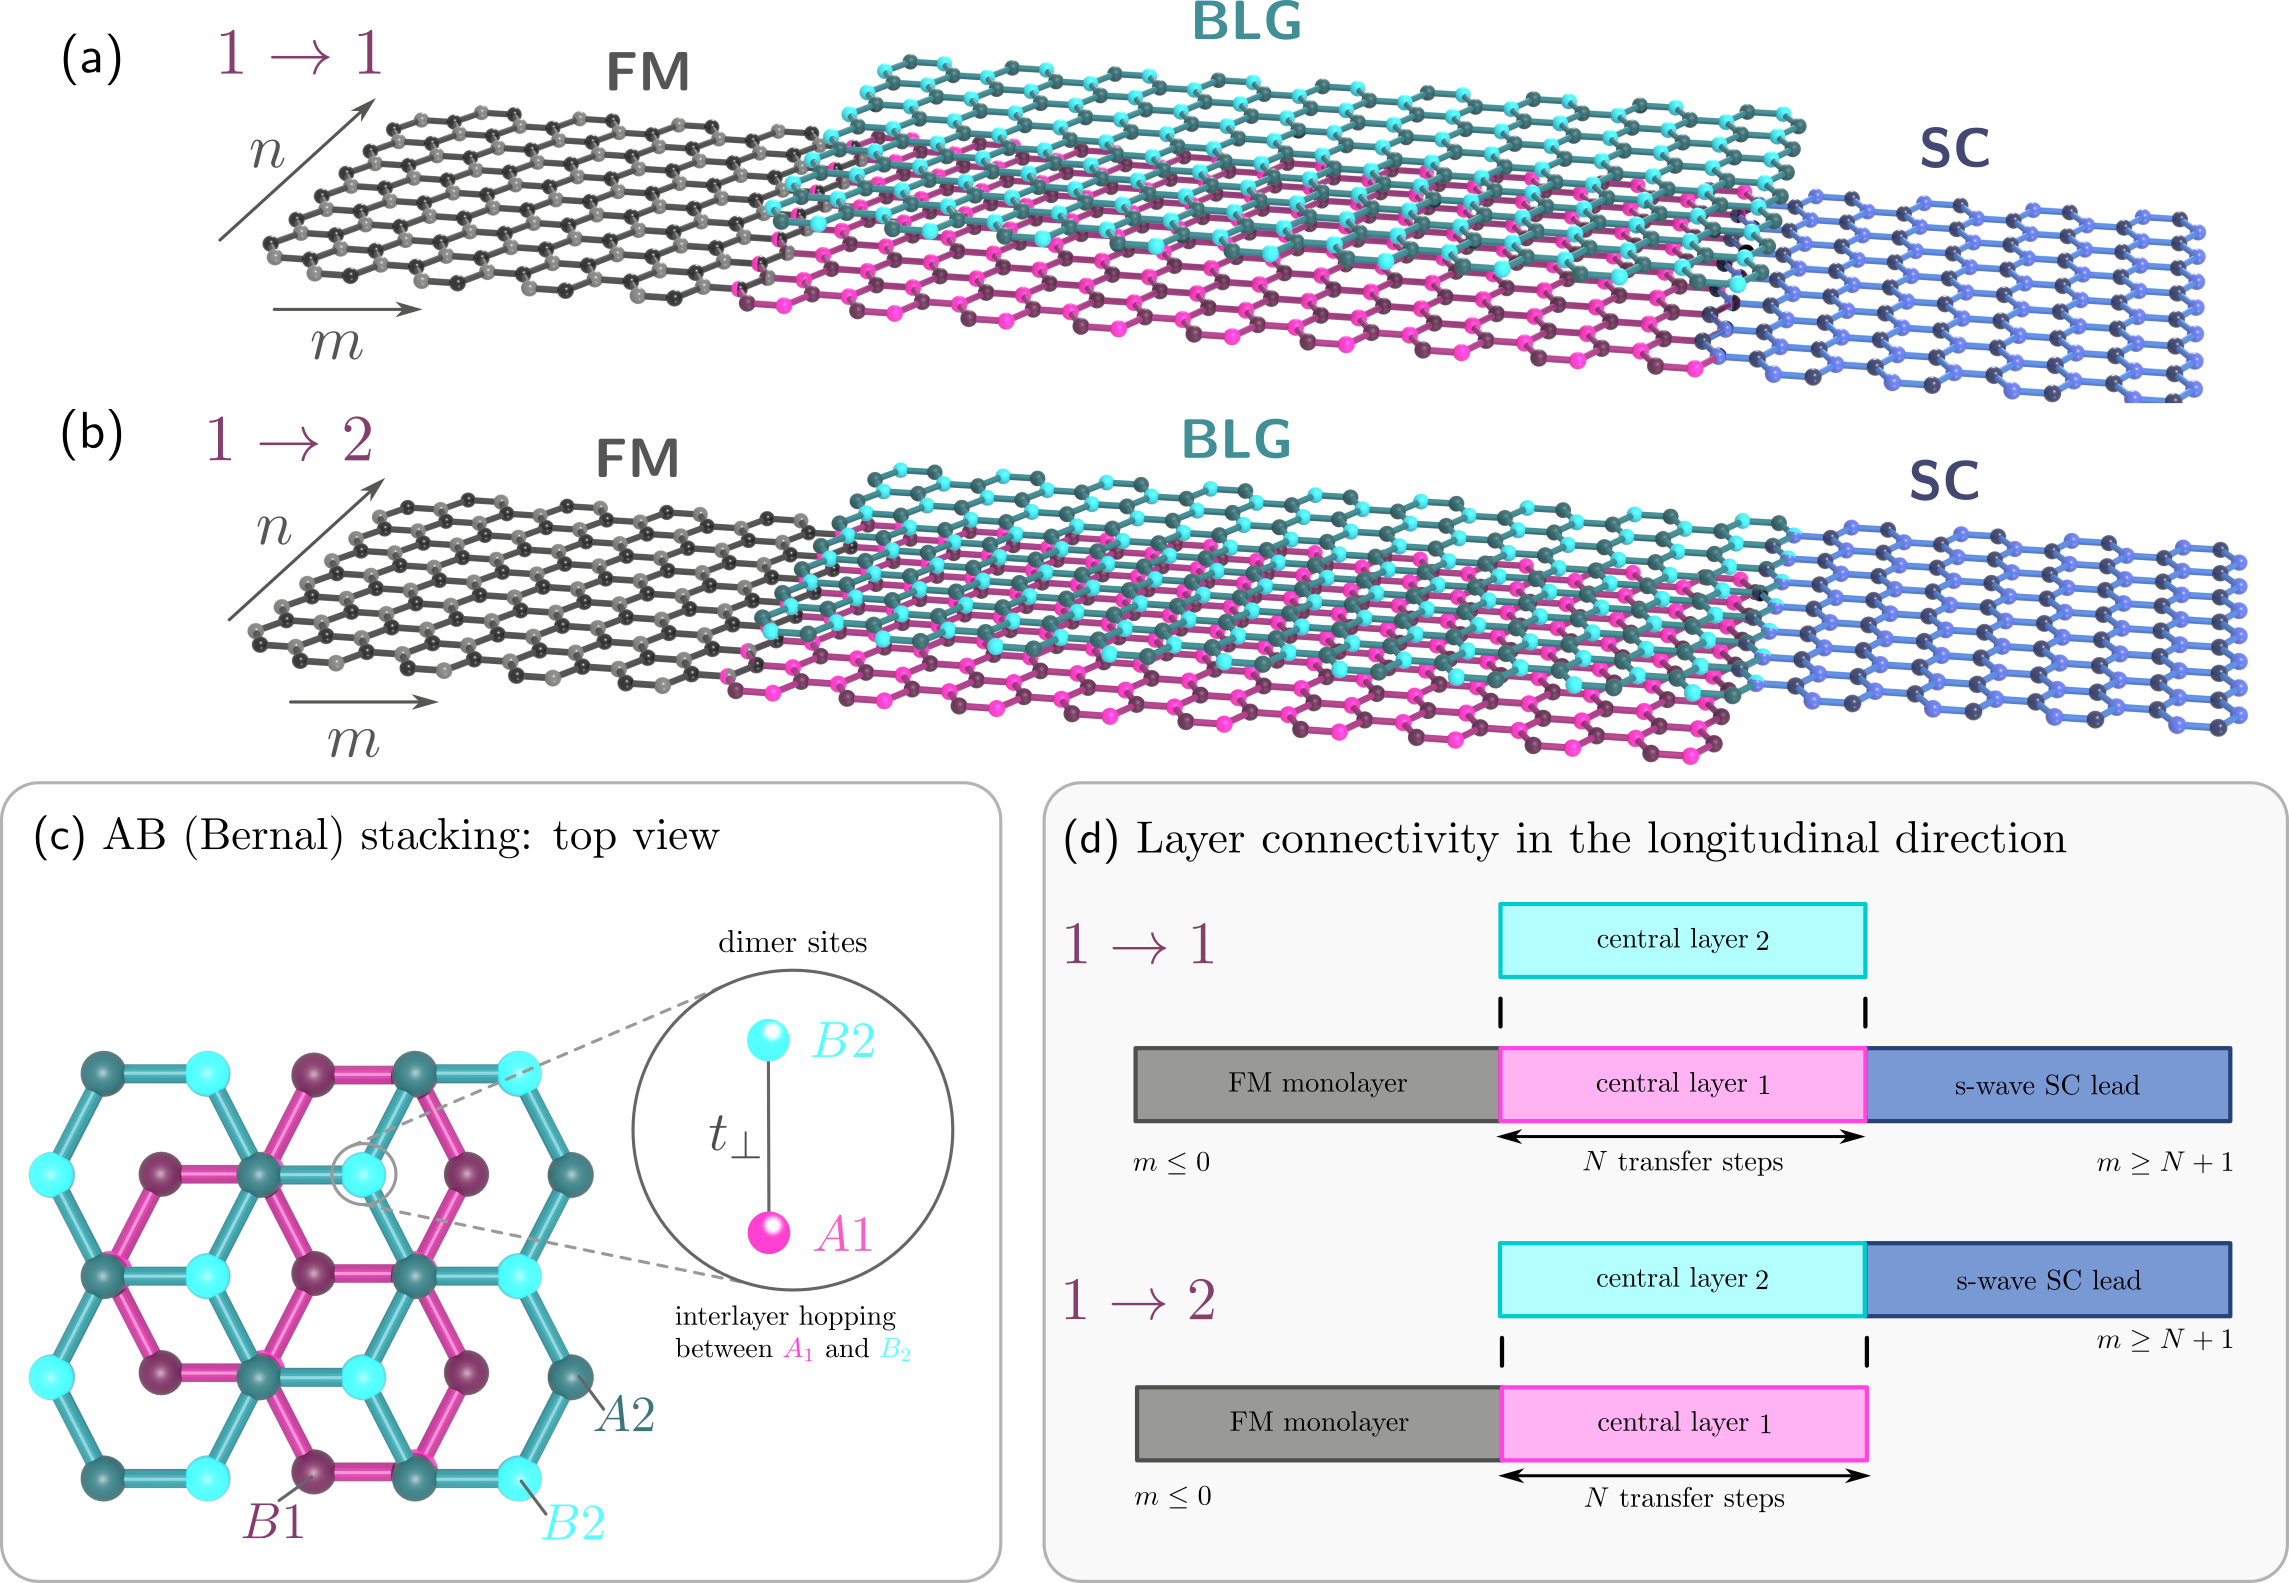
\includegraphics[width=\textwidth]{figures/system.png}
	\caption{\label{figgeometry}\label{fig:geometry}
		Geometry, lattice structure, and longitudinal connectivity of the
		ferromagnet--bilayer-graphene--superconductor (FM--BLG--SC)
		junction.
		(a)~Atomic representation of the $1\!\to\!1$ geometry, in which
		the ferromagnetic (FM) and superconducting (SC) monolayer graphene
		leads are connected to the same layer of the finite bilayer graphene
		(BLG) region.
		(b)~Corresponding $1\!\to\!2$ geometry, in which the FM and SC
		leads are connected to opposite graphene layers.
		The longitudinal and transverse lattice directions are denoted by
		$m$ and $n$, respectively.
		Gray, magenta, cyan, and indigo identify the FM monolayer,
		central layer~1, central layer~2, and SC monolayer, respectively.
		(c)~Top view of the AB (Bernal) stacking in the central bilayer.
		Different shades within each layer distinguish the $A$ and $B$
		sublattices.
		The enlarged detail shows the vertically registered $A_1$ and
		$B_2$ dimer sites, coupled by the interlayer hopping $t_\perp$;
		the $A_1$ site is hidden beneath $B_2$ in the top projection.
		The non-dimer sites $B_1$ and $A_2$ are also indicated.
		(d)~Longitudinal layer-connectivity representation of the
		$1\!\to\!1$ and $1\!\to\!2$ junctions.
		The FM lead occupies $m\leq0$, the finite BLG region extends over
		$N$ transfer steps, $1\leq m\leq N$, and the SC lead occupies
		$m\geq N+1$.
		In the $1\!\to\!1$ geometry the SC lead continues from central
		layer~1, whereas in the $1\!\to\!2$ geometry it continues from
		central layer~2.%
	}
\end{figure*}


The system is illustrated in Fig.~\ref{figgeometry}.  It is composed of two graphene layers, labeled by $j=1,2$, arranged in two contact geometries denoted by $\oneone$ and $\onetwo$, corresponding to Figs.~\ref{figgeometry}(a) and \ref{figgeometry}(b), respectively.  The longitudinal and transverse directions are indexed by the integers $m$ and $n$.  With this convention, the finite bilayer region occupies
\begin{equation}
	1\le m\le N
	\label{eq:central-region}
\end{equation}
in both geometries.  For $m\le0$ the graphene monolayer is ferromagnetic, whereas for $m\ge N+1$ the monolayer is an $s$-wave superconductor.

The main difference between the two geometries concerns the right contact, where the finite bilayer is coupled to the superconducting monolayer.  In the $\oneone$ geometry, the superconductor is coupled to the lower layer, the same layer that is connected to the ferromagnetic monolayer.  In the $\onetwo$ geometry, the ferromagnetic monolayer is still connected to the lower layer, but the superconducting monolayer is coupled to the upper layer.  This distinction is most clearly visualized in the block diagram of Fig.~\ref{figgeometry}(d).  In both geometries we assume Bernal stacking in the central region, as shown in Fig.~\ref{figgeometry}(c), with an $A$ atom of the lower layer coupled to a $B$ atom of the upper layer by the interlayer hopping $t_\perp$.

We now translate this figure-based description into the domains used in the Hamiltonian sums.  The set of layer--cell pairs that physically exist in the $\oneone$ geometry is
\begin{equation}
	\mathcal D_{\oneone}
	=
	\{(1,m):m\in\mathbb Z\}
	\cup
	\{(2,m):1\le m\le N\}.
	\label{eq:domain-11}
\end{equation}
Thus layer~1 extends through the whole junction, while layer~2 exists only in the finite bilayer overlap.  For the $\onetwo$ geometry,
\begin{equation}
	\mathcal D_{\onetwo}
	=
	\{(1,m):m\le N\}
	\cup
	\{(2,m):m\ge 1\}.
	\label{eq:domain-12}
\end{equation}
Thus layer~1 extends from the ferromagnetic lead through the central bilayer and terminates at the right edge, while layer~2 begins at the left edge of the central bilayer and continues into the superconducting lead.  In what follows, $g\in\{\oneone,\onetwo\}$ labels the chosen geometry and $\mathcal D_g$ denotes the corresponding physical domain.

All microscopic sums below are restricted to $(j,m)\in\mathcal D_g$.  A hopping or pairing term is included only if every site appearing in that term belongs to the physical domain.  A missing neighbor at a terminated layer is therefore not assigned a zero amplitude by hand; the corresponding bond is absent from the Hamiltonian.  This convention is the microscopic origin of the termination conditions used later in the interface matching.

The remaining internal labels are the sublattice index $\alpha=A,B$ and the spin label $\sigma=\uparrow,\downarrow$, with
\begin{equation}
	s_\uparrow=+1,
	\qquad
	s_\downarrow=-1.
\end{equation}

\subsection{Real-space tight-binding Hamiltonian}
\label{subsec:hamiltonian}

The microscopic Hamiltonian is written as
\begin{equation}
	\hat H^{(g)}
	=
	\hat H_t^{(g)}
	+
	\hat H_\perp
	+
	\hat H_{\rm on}^{(g)}
	+
	\hat H_\Delta^{(g)} .
	\label{eq:H-total}
\end{equation}
The superscript $(g)$ emphasizes that the intralayer, onsite, and pairing terms depend on the physical domain of the chosen contact geometry.

With the honeycomb convention used in Ref.~\onlinecite{olyaei2019}, each $A$ site is connected to three nearest-neighbor $B$ sites.  The intralayer hopping is
\begin{align}
	\hat H_t^{(g)}
	 & =-t
	\sum_{(j,m)\in\mathcal D_g}
	\sum_{n,\sigma}
	\Big[
		\hat a_{jmn\sigma}^{\dagger}\hat b_{jmn\sigma}
		+
		\hat a_{jmn\sigma}^{\dagger}\hat b_{j,m+1,n,\sigma}
	\notag            \\
	 & \hspace{5.5em}
		+
		\hat a_{jmn\sigma}^{\dagger}\hat b_{j,m,n+1,\sigma}
		+\hc
		\Big].
	\label{eq:H-t}
\end{align}
The longitudinal bond in Eq.~\eqref{eq:H-t} is present only when both $(j,m)$ and $(j,m+1)$ belong to $\mathcal D_g$.

The AB interlayer hopping exists only inside the central bilayer, where both layers are present:
\begin{equation}
	\hat H_\perp
	=
	-t_\perp
	\sum_{m=1}^{N}
	\sum_{n,\sigma}
	\left(
	\hat a_{1mn\sigma}^{\dagger}
	\hat b_{2mn\sigma}
	+\hc
	\right).
	\label{eq:H-perp}
\end{equation}
Thus the dimer bond connects $A_1$ to $B_2$ for $1\le m\le N$.

The onsite normal term is
\begin{equation}
	\hat H_{\rm on}^{(g)}
	=
	\sum_{(j,m)\in\mathcal D_g}
	\sum_{n,\alpha,\sigma}
	\left[ V_j(m)-\mu(m)-s_\sigma h(m)\right]
	\hat n_{jmn\alpha\sigma},
	\label{eq:H-on}
\end{equation}
where
\begin{equation}
	\hat n_{jmn\alpha\sigma}
	=
	\hat c_{jmn\alpha\sigma}^{\dagger}
	\hat c_{jmn\alpha\sigma} .
\end{equation}
Here $\alpha=A,B$ is the sublattice index.  The spatial region is determined by $m$ and by the physical domain $\mathcal D_g$, not by an additional operator label.  The chemical potential is piecewise constant,
\begin{equation}
	\mu(m)=
	\begin{cases}
		\mu_F, & m\le0,       \\
		\mu_C, & 1\le m\le N, \\
		\mu_S, & m\ge N+1,
	\end{cases}
	\label{eq:mu-piecewise}
\end{equation}
and the collinear exchange field is confined to the ferromagnetic lead,
\begin{equation}
	h(m)=
	\begin{cases}
		h, & m\le0, \\
		0, & m\ge1.
	\end{cases}
	\label{eq:h-piecewise}
\end{equation}
The layer potentials $V_1(m)$ and $V_2(m)$ are nonzero only in the central bilayer and allow for layer-resolved gating.

The superconducting lead contains onsite spin-singlet pairing,
\begin{align}
	\hat H_\Delta^{(g)}
	={} &
	\sum_{(j,m)\in\mathcal D_g}
	\sum_{n,\alpha}
	\Big[
		\Delta(m)
		\hat c_{jmn\alpha\uparrow}^{\dagger}
		\hat c_{jmn\alpha\downarrow}^{\dagger}
	\notag               \\
	    & \hspace{5.5em}
		+
		\Delta^*(m)
		\hat c_{jmn\alpha\downarrow}
		\hat c_{jmn\alpha\uparrow}
		\Big].
	\label{eq:H-pair}
\end{align}
where
\begin{equation}
	\Delta(m)=
	\begin{cases}
		0,                     & m\le N,   \\
		\Delta_0 e^{i\varphi}, & m\ge N+1.
	\end{cases}
	\label{eq:Delta-piecewise}
\end{equation}
Because the sum in Eq.~\eqref{eq:H-pair} is restricted to $\mathcal D_g$, the pair potential is placed only on the layer that physically continues into the superconducting lead.

\subsection{Fourier-space Hamiltonian}
\label{subsec:fourier-hamiltonian}

We now use translational invariance along the transverse direction to write the model in momentum space.  For $N_y$ transverse cells with periodic boundary conditions, define the dimensionless transverse momentum $K=k_y a_y\in[-\pi,\pi]$ and use
\begin{align}
	\hat a_{jmn\sigma}
	 & =
	\frac{1}{\sqrt{N_y}}
	\sum_K e^{iKn}\hat a_{jmK\sigma},
	\notag \\
	\hat b_{jmn\sigma}
	 & =
	\frac{1}{\sqrt{N_y}}
	\sum_K e^{iKn}\hat b_{jmK\sigma}.
	\label{eq:fourier-convention}
\end{align}
The two intralayer bonds that do not change $m$ combine into the effective intracell hopping
\begin{equation}
	\eta(K)=t(1+e^{iK}),
	\qquad
	\xi=t,
	\label{eq:eta-xi}
\end{equation}
where $\xi$ denotes the longitudinal hopping across one transfer step.  The intralayer term becomes
\begin{align}
	\hat H_t^{(g)}(K)
	 & =-
	\sum_{(j,m)\in\mathcal D_g}
	\sum_\sigma
	\Big[
		\eta(K)
		\hat a_{jmK\sigma}^{\dagger}
		\hat b_{jmK\sigma}
	\notag            \\
	 & \hspace{5.5em}
		+
		\xi
		\hat a_{jmK\sigma}^{\dagger}
		\hat b_{j,m+1,K,\sigma}
		+\hc
		\Big].
	\label{eq:H-t-K}
\end{align}
As in real space, the longitudinal bond is included only when the two sites connected by it exist in $\mathcal D_g$.

The interlayer hopping is diagonal in $K$ because the dimer bond is vertical within the same cell:
\begin{equation}
	\hat H_\perp(K)
	=
	-t_\perp
	\sum_{m=1}^{N}
	\sum_\sigma
	\left(
	\hat a_{1mK\sigma}^{\dagger}
	\hat b_{2mK\sigma}
	+\hc
	\right).
	\label{eq:H-perp-K}
\end{equation}
The onsite normal term is also diagonal in $K$,
\begin{equation}
	\begin{split}
		\hat H_{\rm on}^{(g)}(K)
		={} &
		\sum_{(j,m)\in\mathcal D_g}
		\sum_{\alpha,\sigma}
		\left[ V_j(m)-\mu(m)-s_\sigma h(m)\right]
		\\
		    & \times
		\hat n_{jmK\alpha\sigma}.
	\end{split}
	\label{eq:H-on-K}
\end{equation}

The pairing term is different: because it contains two creation or two annihilation operators at the same transverse cell, it couples opposite transverse momenta,
\begin{align}
	\hat H_\Delta^{(g)}(K)
	 & =
	\sum_{(j,m)\in\mathcal D_g}
	\sum_\alpha
	\Big[
		\Delta(m)
		\hat c_{jmK\alpha\uparrow}^{\dagger}
		\hat c_{jm,-K,\alpha\downarrow}^{\dagger}
	\notag            \\
	 & \hspace{5.5em}
		+
		\Delta^*(m)
		\hat c_{jm,-K,\alpha\downarrow}
		\hat c_{jmK\alpha\uparrow}
		\Big].
	\label{eq:H-pair-K}
\end{align}
Thus the normal part is diagonal in $K$, while the singlet-pairing part closes only after $K$ and $-K$ are treated together.  The independent scattering channel labeled by $K$ is therefore the BdG sector
\begin{equation}
	(K,\sigma)\oplus(-K,-\sigma),
	\label{eq:paired-sector}
\end{equation}
not an ordinary normal-state single-momentum block.  In this sense the Hamiltonian is block diagonal in paired BdG sectors; no additional independent sum over $-K$ is introduced when the scattering problem is solved at fixed $K$.
